% !TEX TS-program = XeLaTeX
% use the following command:
% all document files must be coded in UTF-8
\documentclass[english]{textolivre}
% build HTML with: make4ht -e build.lua -c textolivre.cfg -x -u article "fn-in,svg,pic-align"

\journalname{Texto Livre}
\thevolume{15}
%\thenumber{1} % old template
\theyear{2022}
\receiveddate{\DTMdisplaydate{2022}{7}{13}{-1}} % YYYY MM DD
\accepteddate{\DTMdisplaydate{2022}{8}{5}{-1}}
\publisheddate{\DTMdisplaydate{2022}{9}{21}{-1}}
\corrauthor{Cláudia de Barros}
\articledoi{10.35699/1983-3652.2022.40454}
%\articleid{NNNN} % if the article ID is not the last 5 numbers of its DOI, provide it using \articleid{} commmand 
% list of available sesscions in the journal: articles, dossier, reports, essays, reviews, interviews, editorial
\articlesessionname{dossier}
\runningauthor{De Barros} 
%\editorname{Leonardo Araújo} % old template
\sectioneditorname{Daniervelin Pereira}
\layouteditorname{Leonado Araújo}

\title{Neuromethodology and neuroimaging for a teacher training}
\othertitle{Neurometodologia e neuroimagem para a formação de professores}
% if there is a third language title, add here:
%\othertitle{Artikelvorlage zur Einreichung beim Texto Livre Journal}

\author[1]{Claudia de Barros \orcid{0000-0002-2286-8674} \thanks{Email: \href{mailto:claudia.barros@uam.es}{claudia.barros@uam.es}}}
\affil[1]{Universidad Autónoma de Madrid, Facultad de Formación de Profesorado y de la Educación, Departamento Pedagogía, Madrid, España.}

\addbibresource{article.bib}
% use biber instead of bibtex
% $ biber article

% used to create dummy text for the template file
\definecolor{dark-gray}{gray}{0.35} % color used to display dummy texts
\usepackage{lipsum}
\SetLipsumParListSurrounders{\colorlet{oldcolor}{.}\color{dark-gray}}{\color{oldcolor}}

% used here only to provide the XeLaTeX and BibTeX logos
\usepackage{hologo}

% if you use multirows in a table, include the multirow package
\usepackage{multirow}

% provides sidewaysfigure environment
\usepackage{rotating}

% CUSTOM EPIGRAPH - BEGIN 
%%% https://tex.stackexchange.com/questions/193178/specific-epigraph-style
\usepackage{epigraph}
\renewcommand\textflush{flushright}
\makeatletter
\newlength\epitextskip
\pretocmd{\@epitext}{\em}{}{}
\apptocmd{\@epitext}{\em}{}{}
\patchcmd{\epigraph}{\@epitext{#1}\\}{\@epitext{#1}\\[\epitextskip]}{}{}
\makeatother
\setlength\epigraphrule{0pt}
\setlength\epitextskip{0.5ex}
\setlength\epigraphwidth{.7\textwidth}
% CUSTOM EPIGRAPH - END

% LANGUAGE - BEGIN
% ARABIC
% for languages that use special fonts, you must provide the typeface that will be used
% \setotherlanguage{arabic}
% \newfontfamily\arabicfont[Script=Arabic]{Amiri}
% \newfontfamily\arabicfontsf[Script=Arabic]{Amiri}
% \newfontfamily\arabicfonttt[Script=Arabic]{Amiri}
%
% in the article, to add arabic text use: \textlang{arabic}{ ... }
%
% RUSSIAN
% for russian text we also need to define fonts with support for Cyrillic script
% \usepackage{fontspec}
% \setotherlanguage{russian}
% \newfontfamily\cyrillicfont{Times New Roman}
% \newfontfamily\cyrillicfontsf{Times New Roman}[Script=Cyrillic]
% \newfontfamily\cyrillicfonttt{Times New Roman}[Script=Cyrillic]
%
% in the text use \begin{russian} ... \end{russian}
% LANGUAGE - END

% EMOJIS - BEGIN
% to use emoticons in your manuscript
% https://stackoverflow.com/questions/190145/how-to-insert-emoticons-in-latex/57076064
% using font Symbola, which has full support
% the font may be downloaded at:
% https://dn-works.com/ufas/
% add to preamble:
% \newfontfamily\Symbola{Symbola}
% in the text use:
% {\Symbola }
% EMOJIS - END

% LABEL REFERENCE TO DESCRIPTIVE LIST - BEGIN
% reference itens in a descriptive list using their labels instead of numbers
% insert the code below in the preambule:
%\makeatletter
%\let\orgdescriptionlabel\descriptionlabel
%\renewcommand*{\descriptionlabel}[1]{%
%  \let\orglabel\label
%  \let\label\@gobble
%  \phantomsection
%  \edef\@currentlabel{#1\unskip}%
%  \let\label\orglabel
%  \orgdescriptionlabel{#1}%
%}
%\makeatother
%
% in your document, use as illustraded here:
%\begin{description}
%  \item[first\label{itm1}] this is only an example;
%  % ...  add more items
%\end{description}
% LABEL REFERENCE TO DESCRIPTIVE LIST - END


% add line numbers for submission
%\usepackage{lineno}
%\linenumbers

\begin{document}
\maketitle

\begin{polyabstract}
\begin{abstract}
Neuromethodology is a concept about which we hardly find information in scientific databases and specialized literature. Therefore, the general objective of the study presented is to analyze the relationship between teaching methodology, teaching neuromethodology, educational inclusion, technology and teacher training. The research design is non-experimental, descriptive, explanatory, correlational and regression. The sample used was, by convenience, taken from university teachers from Spanish, Brazilian, Colombian and Paraguayan universities, with a number of 815 participants. The research instrument was an \textit{ad hoc} Likert scale questionnaire with excellent reliability (Cronbach's Alpha, .969), which was validated in content and construct through an exploratory factor analysis. Correlation analysis and automatic linear modeling provide a first conclusion showing that neuromethodology gives scientificity to the technologies used by the teacher, being fundamental for educational inclusion. The neuroimaging examples provide an idea of the research we are developing in neuromethodology.

\keywords{Teaching Methodology \sep Teaching Neuromethodology \sep Neuroimaging \sep Teacher Training \sep Brain}
\end{abstract}

\begin{portuguese}
\begin{abstract}
A neuromethodologia é um conceito sobre o qual dificilmente encontramos informações em bancos de dados científicos e literatura especializada. Portanto, o objetivo geral do trabalho apresentado é analisar a relação entre metodologia de ensino, ensino de neuromethodologia, inclusão educacional, tecnologia e formação de professores. O projeto da pesquisa é não-experimental, descritivo, explicativo, correlacional e regressivo. A amostra utilizada foi uma amostra de conveniência de professores universitários de universidades espanholas, brasileiras, colombianas e paraguaias, com um total de 815 participantes. O instrumento de pesquisa foi um questionário \textit{ad hoc} à escala Likert com excelente confiabilidade (Cronbach's Alpha, .969), que foi validado em termos de conteúdo e construído através de uma análise exploratória de fatores. A análise de correlação e a modelagem linear automática fornecem uma primeira conclusão mostrando que a neuromethodologia dá cientificidade às tecnologias utilizadas pelo professor, sendo fundamental para a inclusão educacional. Os exemplos de neuroimagem dão uma ideia da pesquisa que estamos desenvolvendo em neuromethodologia.

\keywords{Metodologia de ensino \sep Neuromethodologia de ensino \sep Neuroimagem \sep Treinamento de professores \sep Cérebro}
\end{abstract}
\end{portuguese}
% if there is another abstract, insert it here using the same scheme
\end{polyabstract}

\section{Introduction}\label{sec-intro}
The present study has as its theme teaching methodology, educational inclusion, technology and teacher training, in their relationship with teaching neuromethodology, a term that we will try to delimit in this research and illustrate, within the scientific field of neuropedagogy, through neuroimaging techniques. We begin by defining and highlighting the main ideas of the topics to be investigated.

Methodology is literally the doctrine of the method, but the method already implies in itself to be practical teaching, wanting to define it falls into tautology. Methodology involves the study of acts of reason and logic, being this study speculative and practical at the same time. Methodology, then, can be defined as practical logic \cite[p. 1288]{varios_enciclopedia_1917}. According to \textcite[p. 320]{neuner_pedagogi_1981} the teaching method is "a system of actions of the teacher aimed at organizing the practical and cognitive activity of the student with the objective of solidly assimilating the contents of education". According to \textcite[p. 85]{zabalza_beraza_metodologidocente_2011}, talking about methodology implies not only "determining what are going to be the things we are going to do with our students, but also assuming under what approach we are going to approach this joint work. It is, therefore, more a conceptual than an operational problem". On the other hand, to study methodology is to confront "a complex space of variables that intertwine and mutually condition each other. Methodology is a kind of meeting point of doctrinal and practical dimensions, of traditions and regulations, of institutional positions and individual stances. In this network of influences, there is a risk of being left with partial and scarcely relevant visions" \textcite[p. 85]{zabalza_beraza_metodologidocente_2011}. With all this, it is interesting to highlight the components of the methodology, according to \textcite{zabalza_beraza_metodologidocente_2011} and which we assume here: 

\begin{itemize}
    \item Organization of spaces and times;
    \item The way information is provided;
    \item The orientation and management of learning activities;
    \item Interpersonal relationships.
\end{itemize}

The teaching methodology, following the educational guidelines of the major international organizations, must be inclusive, or at least have educational inclusion as a methodological reference. Consequently, we will now detail the topic of inclusion. \textcite[p. 27]{arnaiz_reto_1996} points out that inclusive education "is an attitude, a system of values and beliefs, not an action or a set of actions". Following \textcite{booth_index_2000}, the development of Inclusive Education should be directed towards the fulfillment of several purposes, raised from several interrelated perspectives such as culture, policies and practices of schools and educational institutions. Under this thinking, we can say that the need to create inclusive schools will imply creating a safe, welcoming, collaborative and stimulating school community in which each person is valued, as the primary foundation for all students to have a higher level of success. It proposes the development of inclusive values, which are shared by the whole school group, whose derived ideas guide the decisions that are concretized in the school policies of each educational institution and in the educational day-to-day, and in this way the learning of all people finds support in the continuous process of educational innovation.

As well as educational inclusion, teaching methodology must assume technologies as a resource and as a field of knowledge, which is why this research topic will be detailed below. \textcite[p. 1]{de_la_orden_hoz_tecnologieducativa_1986} says that:
\begin{quote}
    originally, educational technology was presented as a discipline whose main objective was focused on the study of technical instruments and equipment and their different forms of school use, considering these instruments as a vehicle or support for various didactic functions, especially the presentation of stimuli and content to students.
\end{quote}

The basis of this technology was constituted by the audiovisual media: cinema, still image, sound regisuo, radio, etc., which had been developing since the end of World War II. According to \textcite{jimenez_metodologiinvestigacion_2008} technology is defined as "the result of knowledge that allows the production of artifacts or processes, modifies the environment, including plants and animals, to generate welfare and satisfy human needs". \textcite{nunez_siglo_1999} considers that we can find several conceptions about this terminology. In one of them, technology is conceived in terms of its scientific appearance, i.e., knowledge, skills, instruments and devices. In another, the term technology also incorporates the distributive vision, economic practice and manufacture, labor work, beneficiary, consumers and the educational vision, which involves the purposes, aptitudes, moral keys and regulations of conduct.

Summarizing what has been exposed so far, it can be observed that the teaching methodology must be well characterized, inclusive and with technological features, which implies assuming training processes in teachers. In fact the training of teachers is a historical concern, and we can  asume it is most important problem in the context of an educational system. The way in which teachers must access their training (objectives, method, etc.) is conditioned by the mode of orientation that will shape the institution that is needed. In history, any alteration in an educational center is shown, not only from the concern for transmitting knowledge, but also for its incorporation in the fundamental cultural areas that are the basis of a system characterized by its innovation. All of the above fully affects training models and training centers, which in one way or another seek to be consistent with the dominant ideas of each historical moment. The purpose of training is "knowing how to analyze", understanding the concept as a unique learning that restructures the act and collaborates in new learning. \textcite{stenhouse_investigacion_1987} places great value on the idea that training is an activity of inquiry, through which teachers can reflect on their unique activity and use the results of their own activity to increase the quality of teaching. L'hotellier points out that "training is the ability to transform everyday events into meaningful experience, within the horizon of a personal and collective project" \cite[p. 20]{honore_para_1980}. Therefore, training is not something that is acquired once and for all, that is the possession of some, or that is achieved only with a professional degree; it is a kind of function proper to the human being, which is cultivated and can be developed, which is not subject to specific temporalities or ages. It is an evolutionary function that is exercised according to a certain process and triggers the constitutive experience of being. 

Together with educational inclusion and technology, neuroscientific studies and their application in education through neuroeducation have emerged strongly in recent decades, imposing a field of study in any educational aspect to be investigated. In this order of things, methodology cannot be alien to these advances. In this paper we think that it can be assumed that the teaching methodology acquires neuroscientific resources to enrich itself, or, alternatively, to evolve the methodology to neuromethodology and establish a new field of study. If we search for the term "neuromethodology" in the Scopus database, we do not find any results, as in the other scientific databases, so we are faced with a scientific field to be developed.

Neuroimaging is increasingly used in research because it provides a dynamic view of brain function. The measurement of brain electrical activity with non-invasive electrodes allows us to obtain neurophysiological information under different conditions. The brain-computer interface (BCI) used in this work, to exemplify the lines of research that we will follow in future publications, has been emotiv, which uses four of the five bands expressed by \textcite{cardinali_neurociencia_2007}: theta (4 to 8 Hz), alpha (8 to 12 Hz), beta (14 to 30Hz) and gamma (30 to 80 Hz).

\section{Method}\label{sec-normas}
The general objective of this research is to analyze the relationship between teaching methodology, teaching neuromethodology, educational inclusion, technology and teacher training. The research design is non-experimental, descriptive, explanatory and correlational, with a quantitative methodology. The research instrument was a questionnaire, Likert scale type, created \textit{ad hoc}.

The sample constituted by convenience of university professors, with a Master's degree and/or doctorate, and professional category of doctoral assistant, hired doctor, tenured university professor or professor, from Spanish, Brazilian, Colombian and Paraguayan universities. The total number of participants was 815, 575 from Spain, 144 from Brazil, 48 from Colombia and 48 from Paraguay.

The questionnaire was constructed with the corresponding operationalization table, with five dimensions and 26 items. This instrument was validated in its content, through a judgment of 12 experts (doctors specialized in the subject) and a pilot test applied to a part of the sample, where some grammatical alterations were made in the items, after which, it was considered validated in content.

\section{Results}\label{sec-conduta}
The first noteworthy result comes from the validation of the construct of the data collection instrument; thus, an exploitative factor analysis was performed. 

Construct validity (Exploratory Factor Analysis).

\begin{itemize}
    \item Correlation matrix study: to check the correlation matrix we have used the Kaiser Meyer Olkin measure of sampling adequacy (KMO coefficient) -- in our case the value is 0.923. Following \textcite[p. 35]{kaiser_index_1974} the value is good, Bartlett's sphericity test has a significance of .000, and the value of the determinant is 6.789E-32, so we continued with the analysis.
    \item Extraction of the factors: the communalities graph shows that the factors have a value greater than .594 so it is not necessary to eliminate any item from the factor analysis. 
    
    The best represented items are: C13.-Educational inclusion is an attitude, a system of values and beliefs, not an action or a set of actions (.937). A2.-Strategies (cooperative, collaborative learning...) are a component of the teaching methodology (.935). E25.-Educational inclusion is key in teacher training (.927).The worst represented item is: C16.-Technologies favor educational inclusion (.594).
    \item Factor rotation: in our case these are the first 6 factors, which explain 86.432 \% of the accumulated variance.
    \item Study of the factorial scores: Factor I: Dimension A: A1.-The teaching methodology is a system of teaching actions that allow organizing the practical and cognitive activity of the students so that they can assimilate the educational contents. A2.-The strategies (cooperative, collaborative learning...) are a component of the teaching methodology. A3.-The techniques (group, individual...) are key in the teaching methodology. A4.-The instruments (teaching-learning materials) are very important in the teaching methodology. Dimension B: B6.-Teaching neuromethodology is the set of methods, strategies, techniques, instruments and resources that, with a neurodidactic basis, allow the development of teaching practice. B7.-Strategies such as problem-based learning, project-based learning, collaborative learning, etc., should be transformed into teaching neuromethodologies. B8.-Teaching methods (deductive, analytical...) should be transformed into neuromethods. Techniques, instruments and resources must acquire neurodidactic aspects. Educational inclusion needs neuromethodology. Neuromethodology gives scientificity to the technologies used by the teacher. B12.-Training in teaching neuromethodology is essential. Dimension C: C14.-Teaching methodology favors educational inclusion. C15.-Neuromethodology supports educational inclusion. C16.-Technologies favor educational inclusion. C17.-Teacher training in educational inclusion is needed. Dimension D: D18.-By technologies we mean the discipline whose fundamental objective is centered on the study of technical instruments and equipment and their different forms of school use, considering these instruments as a vehicle or support for various functions. D19.-The teaching methodology favors the application of technologies in schools. D20.-Neuromethodology supports the use of technologies in schools. D21.-Teaching training in technologies is necessary. Dimension E: E22.-Teacher training is the ability to transform daily events into meaningful experience, within the horizon of a personal and collective project. E24.-Neuromethodology is the basis for teacher training. E25.-Educational inclusion is key in teacher training. E26.-Technologies are key in teacher training.
\end{itemize}

We have taken factor 1 (the rest does not have acceptable reliability), which presents a reliability similar to the original scale (.969, 26 items) with three less items (.966, 23 items). 

To perform the correlation, we subjected the Likert scale to the Kruskal-Wallis test to five independent samples, which shows a normal data distribution, so we will perform the Pearson correlation.

Next, we will show the correlations between dimensions that have significant value (0.05):

\begin{itemize}
    \item A.-Teaching methodology correlates significantly with C.-Educational inclusion (.828).
    \item B.-Teaching neuromethodology correlates significantly with D.-Technologies and vice versa (.915).
    \item C.-Educational inclusion correlates significantly with D.-Technologies (.866).
    \item E.-Teacher training correlates significantly with C.-Educational inclusion (.737).
\end{itemize}

Finally, an automatic linear model has been carried out, with the intention of being able to establish how the variable "neuropedagogy" will behave according to the interaction of the rest of the variables. With this, "neuropedagogy" has been taken as the objective and the variable "degree of training" as the analysis weight. The resulting model has an accuracy of 100\% (\Cref{fig01}), showing the weight, from highest to lowest, of the variables that will influence, thus:
The most influential is: B6.-Teaching neuromethodology is the set of methods, strategies, techniques, instruments and resources, based on neurodidactics, that allow the development of teaching practice.

Followed by:

C15.-Neuromethodology is the basis for educational inclusion.

B7.-Strategies such as problem-based learning, project-based learning, collaborative learning, etc., should be transformed into teaching neuro-strategies.

E26.-Technologies are key in teacher training.

B9.-Techniques, tools and resources must acquire neurodidactic aspects.

\begin{figure}[h!]
 \centering
 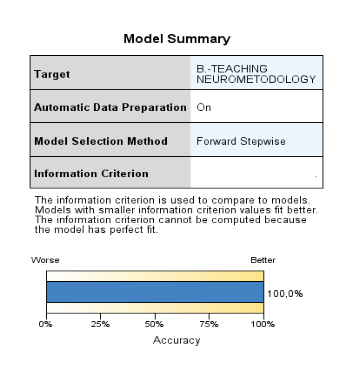
\includegraphics[width=0.85\textwidth]{fig1.png}
 \caption{Automatic linear model.}
 \label{fig01}
 \source{Own elaboration.}
\end{figure}

\section{Neuroimaging in neuromethodology}\label{sec-fmt-manuscrito}
The methodology is easy to observe in a teacher in his classroom activity. However, if what we want is to see the neuromethodology, we must resort to portable neuroimaging, because the ideal is to analyze the brain functioning of the teacher in his natural environment. We show below some examples of brain functioning of a teacher using different methodologies. We must clarify that the examples shown here require some previous conditions, so the person who handles the BCI must have, firstly, neuroscientific, neuroeducational and neuropedagogical  knowledge; secondly a specific training in brain waves and their interpretation; thirdly to know the neurodidactic networks present in the pedagogical processes; and finally to have the appropriate training for the use of the BCI \cite{hernandez_neuroimagen_2022}. 

The location of the BCI electrodes is shown below (\Cref{fig02}), as well as the placement of the emotiv on the author (\Cref{fig03}). The research process has been carried out with a female teacher, with ten years of teaching seniority, and experience in school management. The brain imaging has been performed in her usual environment, and her normal activity (the BCI is portable), so her daily work in the classroom is not altered. The brain image corresponding to a traditional methodology (explanation of a concept) (\Cref{fig04}) and to a mobile learning  methodology (using kahoot) (\Cref{fig05}) is shown. In each case we will obtain some neuropedagogical conclusions about the neuroimaging obtained. Logically, we cannot draw general conclusions, but show the lines of research that we are developing in the research groups EMIPE (Universidad Autónoma de Madrid), ProfesioLab (Universidad de Granada), and the University of Jaén in Spain.

\begin{figure}[h!]
 \centering
 \begin{minipage}{.45\textwidth}
 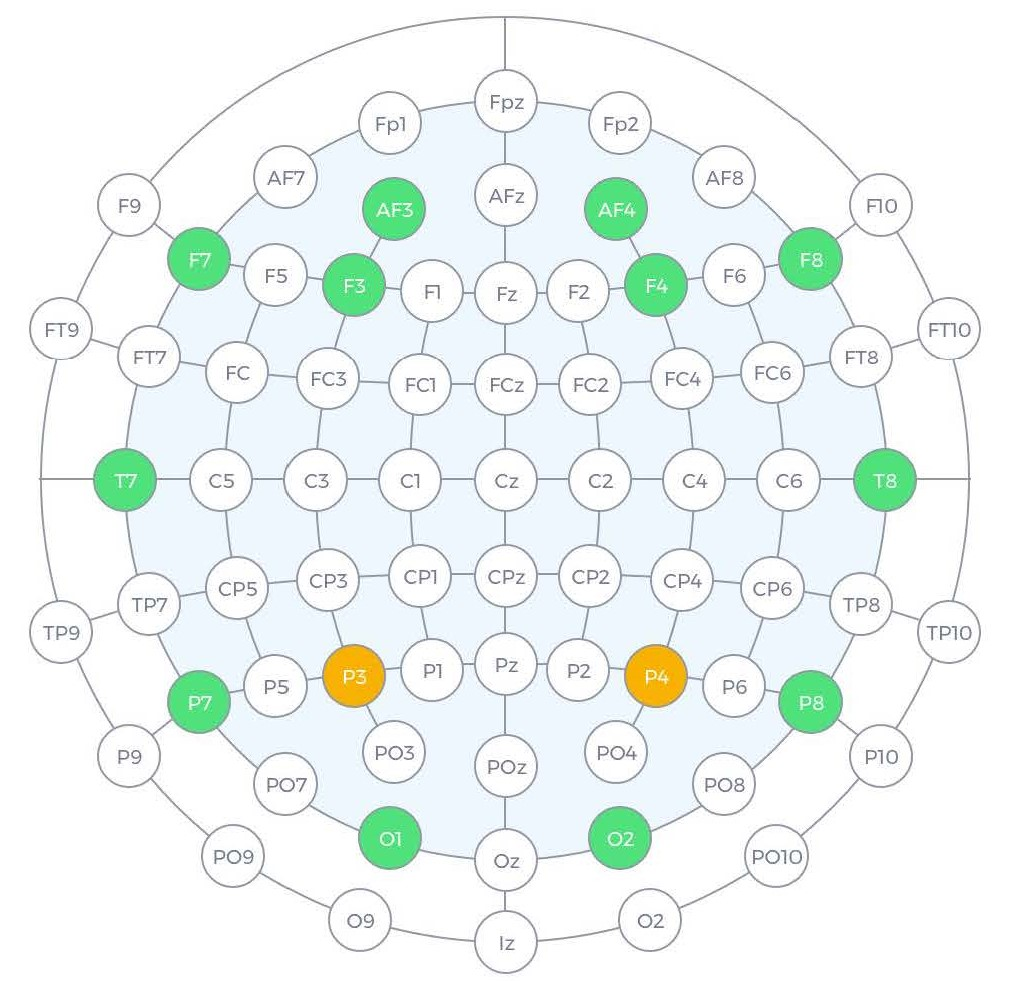
\includegraphics[width=\textwidth]{fig2.png}
 \caption{Location and labeling of the electrodes in emotiv according to the International 10-20 Extended System.}
 \label{fig02}
 \source{\textcite{oostenveld_five_2001}.}
 \end{minipage}%
 \qquad
 \begin{minipage}{0.45\textwidth}
 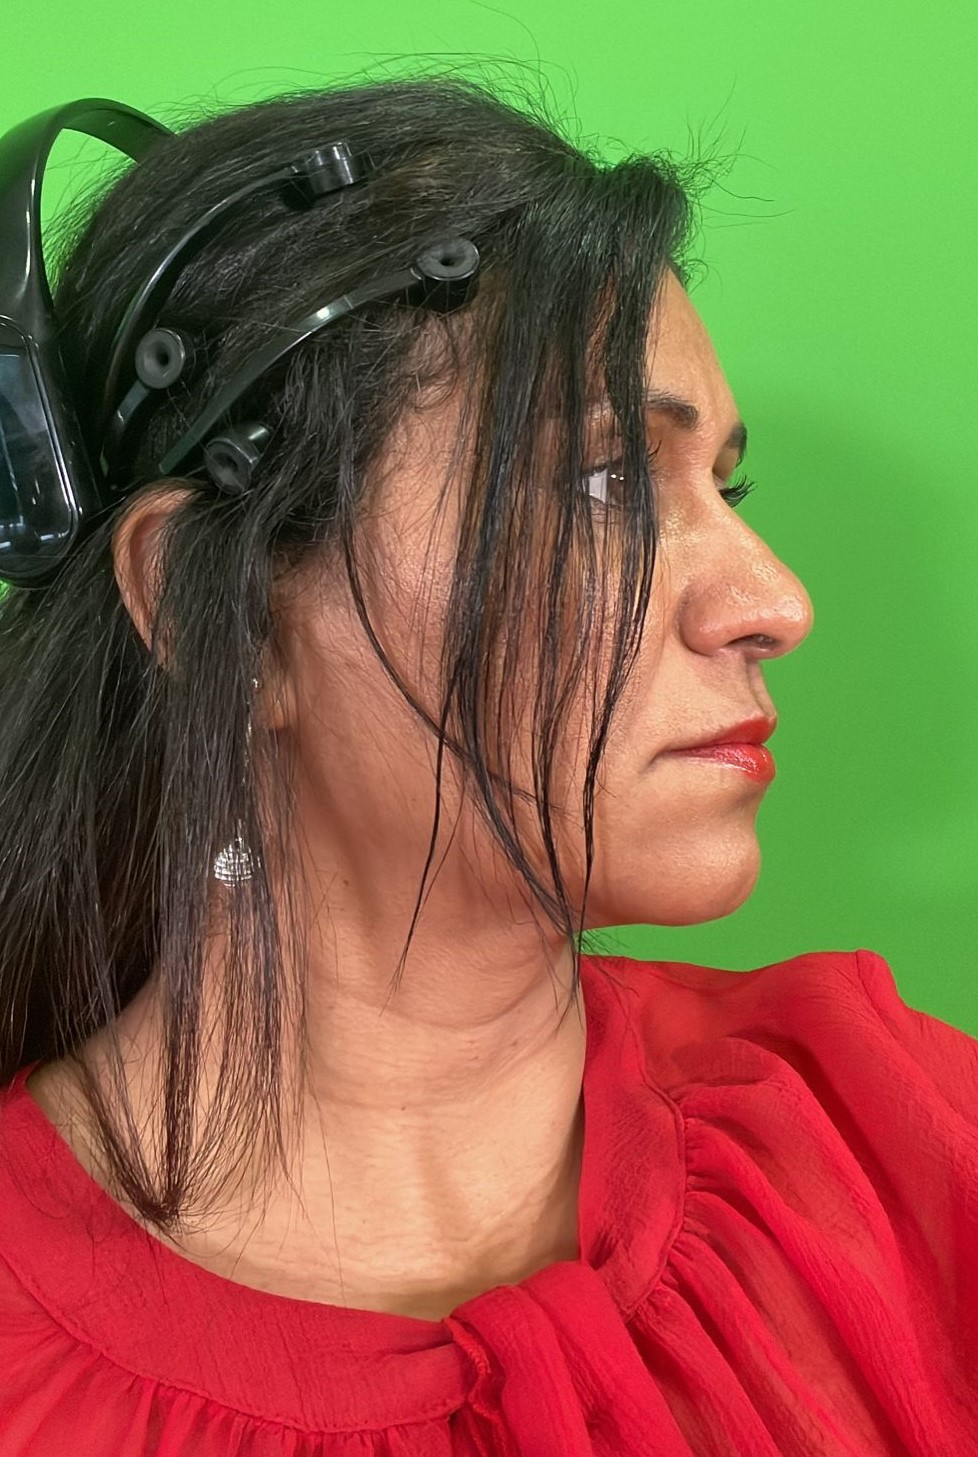
\includegraphics[width=\textwidth]{fig3.png}
 \caption{BCI placement in the author.}
 \label{fig03}
 \source{Own elaboration.} 
 \end{minipage}%
\end{figure}

\begin{figure}[h!]
 \centering
 \begin{minipage}{.45\textwidth}
 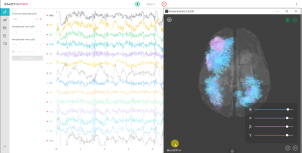
\includegraphics[width=\textwidth]{fig4.png}
 \caption{Methodology – Traditional.}
 \label{fig04}
 \source{Own elaboration.}
 \end{minipage}%
 \qquad
 \begin{minipage}{0.45\textwidth}
 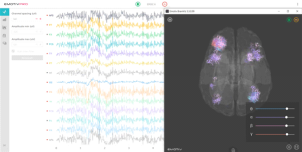
\includegraphics[width=\textwidth]{fig5.png}
 \caption{Methodology – Mobile learning.}
 \label{fig05}
 \source{Own elaboration.} 
 \end{minipage}%
\end{figure}

\begin{figure}[h!]
 \centering
 \begin{minipage}{.45\textwidth}
 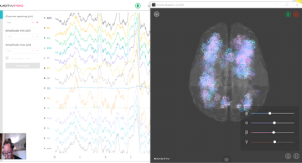
\includegraphics[width=\textwidth]{fig6.png}
 \caption{Female teacher reading a school text.}
 \label{fig06}
 \source{Own elaboration.}
 \end{minipage}%
 \qquad
 \begin{minipage}{0.45\textwidth}
 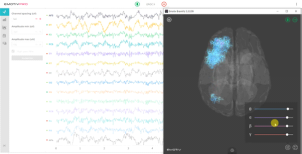
\includegraphics[width=\textwidth]{fig7.png}
 \caption{Male teacher reading a school text.}
 \label{fig07}
 \source{Own elaboration.} 
 \end{minipage}%
\end{figure}

In \Cref{fig04} we observe the teacher in her traditional classroom explanation activity. The neuroimage shows the activation of the left hemisphere (occipital, temporal, parietal and frontal lobe) and curiously the right temporal and occipital lobe. On the contrary, the neuroimaging of an emerging methodology such as the use of mobile learning implies the use of both hemispheres, but with much less intensity. A first conclusion, limited by being a case study, is that the emergent methodology type requires much less brain resources than the traditional class, implying less brainwear on the teacher. The study has been carried out with a female teacher, but what would happen with a male teacher? We pose this question because another line of research that we are opening is the study of gender in the classroom. Just to show a detail, in \Cref{fig06} and \Cref{fig07} we show the neuroimage of the previous teacher reading a regular school text, and the neuroimage of a male teacher, of the same age and similar teaching time. The differences are obvious, so there is no need to insist. With this we ask ourselves: when we do activities in class, do we take into account that boys and girls have different brain processing?

\section{Discussion and conclusions}\label{sec-formato}
The evident absence of studies on neuromethodology justifies the present research, so that in order to relate teaching methodology, educational inclusion, technologies and teacher training with neuromethodology, we have tried to establish the basis for a conceptualization based on empirical evidence. With all this, the exploratory factor analysis shows that educational inclusion, understood as a system of values and beliefs, strategies as components of methodology and educational inclusion as a key to teacher training, are aspects of great weight in the scale. Of less importance is the fact that technologies favor educational inclusion. On the other hand, Pearson's correlation analysis shows that teaching methodology is significantly related to educational inclusion, the latter to technologies and teacher training, and finally, neuromethodology correlates significantly with technologies. With all this, neuromethodology should have in its scope of study and action technology and educational inclusion, for teacher training. To conclude, a statistical regression model has been calculated to predict the evolution of neuromethodology in interaction with the rest of the study dimensions, with an accuracy of 100\%. It can be concluded that neuromethodology gives scientificity to the technologies used by the teacher, being fundamental for educational inclusion; on the other hand, teaching methods (deductive, analytical...) should be transformed into neuromethods, being neuromethodology fundamental for teacher training. However, neuroimaging shows its necessity for neuromethodology research, which, under the vision of neuropedagogy, allows the establishment of new lines of research. We conclude by defining neuromethodology as the set of strategies, methods, techniques, instruments and teaching resources that, with a neuropedagogical basis, integrate technology and inclusion for an innovative and quality education.

\section{Work arising from the projects}
"Formación del Profesorado Universitario en TIC Como Apoyo al Alumnado con Discapacidad". Type of Project/Grant: State Plan 2017-2023 Challenges - R+D+i Projects. Referencia: PID2019-108230RB-I00. 

Included in the Ibero-American Network for the Development of the Professional Identity of Teachers (RED RIDIPD) (University of Jaén, Spain).

Project (2021-1-HR01-KA220-HED-000027562). Autonomous University of Madrid (Spain). Amount of the approved project: 371,219.00 EUR. Duration: 1.2.2022.-31.1.2025. EMIPE Group (Team for interdisciplinary improvement of educational practice). Autonomous University of Madrid.

\printbibliography\label{sec-bib}
% if the text is not in Portuguese, it might be necessary to use the code below instead to print the correct ABNT abbreviations [s.n.], [s.l.]
%\begin{portuguese}
%\printbibliography[title={Bibliography}]
%\end{portuguese}

\end{document}

